\documentclass{article}
\usepackage[utf8]{inputenc}
\usepackage[spanish]{babel}
\usepackage{graphicx}
\usepackage{float}

\title{Práctica 2. Primera parte: Calculadora Sun RPC}
\author{Noelia Escalera Mejías \and Grupo DSD1}

\begin{document}
	\maketitle
	\tableofcontents
	\newpage
	\section{Introducción}
	El primer paso a seguir para implementar la calculadora es escribir el fichero .x ({\it calculadora.x} para nosotros) y luego generar los archivos con {\bf rpcgen -NCa}. Se ha escrito un método para cada operación. He aquí una captura de pantalla del archivo:
	
	\begin{figure}[H]
		\centering
		
\includegraphics[totalheight=11.5cm]{img/2.png}
	\end{figure}
	
	Podemos clasificar las operaciones de la calculadora implementada en 4 grupos: Operaciones básicas, operaciones con vectores, media y operaciones con potencias. Nada más entrar en el programa aparecerá un menú para seleccionar una de ellas:
	\begin{figure}[H]
		\centering
		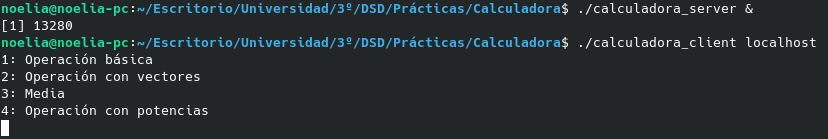
\includegraphics[totalheight=2cm]{img/1.png}
	\end{figure}
	Si introducimos una operación no especificada, nos saltará un mensaje de error y el programa parará su ejecución.
	
	A continuación, hablaremos más en profundidad de cada uno de los distintos grupos de operaciones.
	\section{Operaciones básicas}
	En el guión se especificaba que la calculadora debía hacer operaciones básicas con enteros (sumar, restar, multiplicar y dividir). Sin embargo, en el presente caso se ha tomado la decisión de hacer las operaciones con float para tener más juego. Tenemos entonces, que las operaciones de este bloque son sumar, restar, multiplicar y dividir (ver en el fichero .x o en el del servidor).
	
	Si seleccionamos operaciones básicas en el menú, nos aparece una pequeña ayuda para introducir el formato:
	
	\begin{figure}[H]
		\centering
		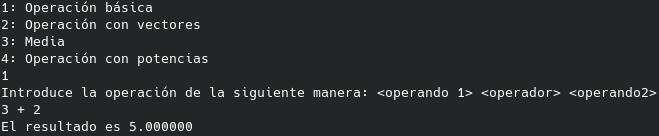
\includegraphics[totalheight=2.5cm]{img/3.png}
	\end{figure}
	Si el formato no es correcto, nos mostrará un mensaje diciendo que la operación no está definida y mostrará en pantalla el resultado 0.
	
	En el cliente simplemente se ha hecho un scanf de los dos operandos y posteriormente un switch del operador. Según el operador escrito, se llamará a una operación del servidor u otra. En el servidor simplemente cada función realiza la operación solicitada con los operandos escogidos. He aquí un ejemplo con la función suma, las diferentes se hacen de manera análoga:
	
	\begin{figure}[H]
		\centering
		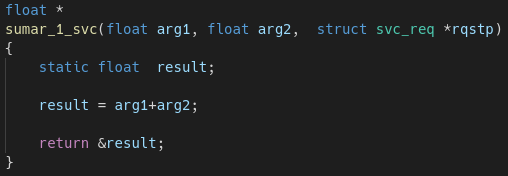
\includegraphics[totalheight=4.2cm]{img/4.png}
	\end{figure}
	\section{Operaciones con vectores}
	Si seleccionamos esta opción, nos aparecerá otro menú con las distintas operaciones que podemos realizar.
	\begin{figure}[H]
		\centering
		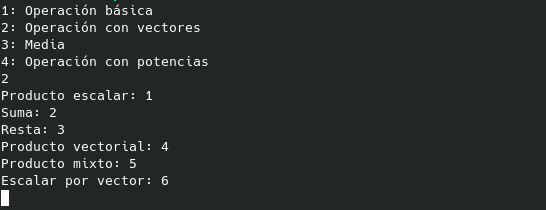
\includegraphics[totalheight=4.5cm]{img/5.png}
	\end{figure}
	El principal problema se ha presentado en esta parte era que no se podían devolver vectores como tal. Se solucionó consultando el foro de dudas de la práctica y usando el typedef t\_vector que se puede observar en el archivo .x. También ha sido necesario crear una variable auxiliar en el cliente de tipo t\_vector para las funciones que devolvían punteros de este tipo en la que copiar el resultado de las operaciones, ya que ha habido problemas a la hora de mostrar los resultados.
	
	\subsection{Producto escalar}
	El producto escalar consiste en multiplicar dos vectores de forma que el resultado sea un escalar. Multiplicamos la coordenada 0 del vector 1 con la coordenada 0 del vector 2, la 1 con la 1, etc y vamos sumando los resultados. He aquí la implementación:
	
	\begin{figure}[H]
		\centering
		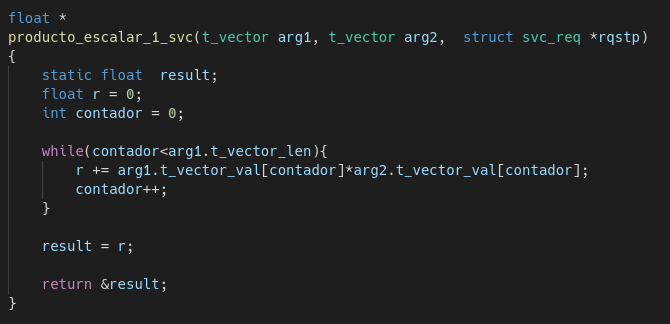
\includegraphics[totalheight=6cm]{img/6.png}
	\end{figure}
	Cuando seleccionamos esta opción en el menú se pedirá una dimensión para los 2 vectores (ya que los 2 deben tener la misma) y a continuación se pedirán los componentes:
	
	\begin{figure}[H]
		\centering
		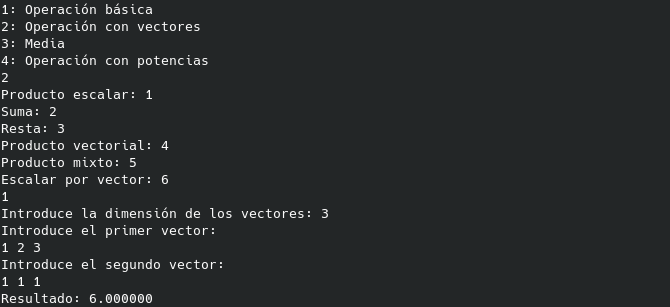
\includegraphics[totalheight=5.5cm]{img/7.png}
	\end{figure}
	Los problemas encontrados aquí han sido con respecto a leer los vectores. Es necesario reservar memoria con malloc al dato t\_vector\_val del vector que se va a leer y actualizar el dato t\_vector\_len. También ha habido problemas con la variable result, al acumular sobre ella cada ejecución (aunque tuviera los mismos datos) daba un valor distino. Para arreglar esto se ha usado la variable r y se ha acumulado sobre ella, copiando su valor final en result.
	\subsection{Suma de vectores}
	Para sumar vectores simplemente hay que sumar las coordenadas de los vectores una a una, de manera que la suma de las coordenadas 0 de los vectores será la coordenada 0 del nuevo vector y así sucesivamente. He aquí la implementación:
	\begin{figure}[H]
		\centering
		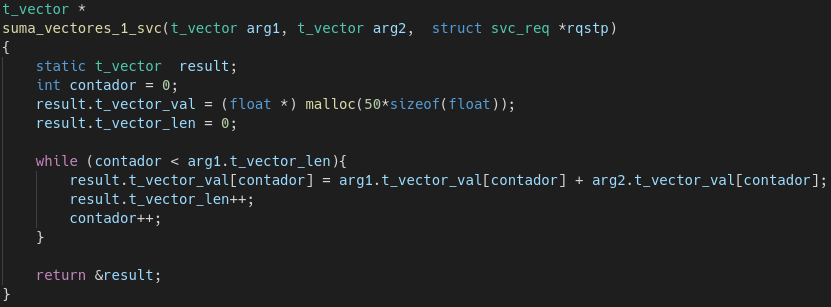
\includegraphics[totalheight=4.6cm]{img/8.png}
	\end{figure}
	El diálogo es prácticamente idéntico al del apartado anterior:
	\begin{figure}[H]
		\centering
		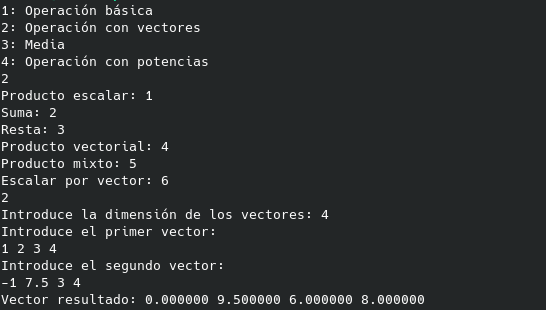
\includegraphics[totalheight=7.2cm]{img/9.png}
	\end{figure}
	\subsection{Resta de vectores}
	Idéntica a la suma de vectores, cambiando sumar por restar.
	\begin{figure}[H]
		\centering
		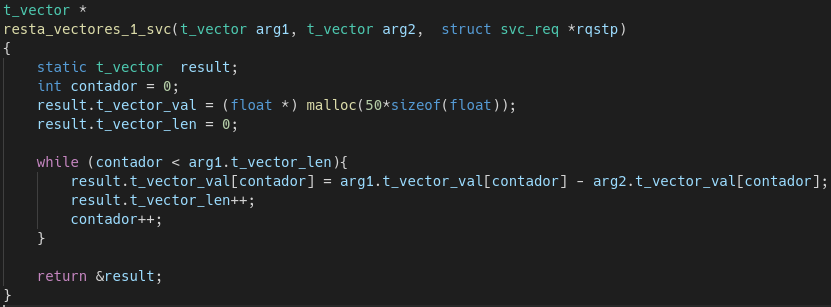
\includegraphics[totalheight=4.7cm]{img/10.png}
	\end{figure}
\begin{figure}[H]
	\centering
	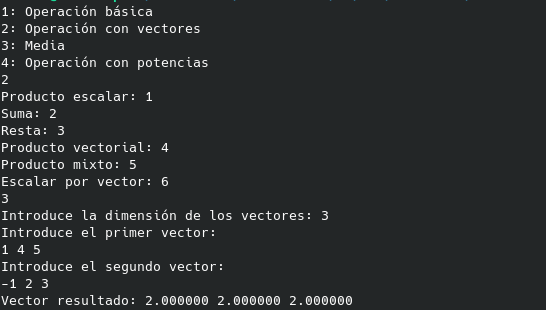
\includegraphics[totalheight=6.8cm]{img/11.png}
\end{figure}
	\subsection{Producto vectorial}
	A diferencia del producto escalar, el resultado del producto vectorial es un vector. Lo que hace es calcular un vector perpendicular a los 2 vectores dados, es por eso que no tiene sentido que los vectores tengan una dimensión mayor que 3. Se calcula resolviendo el siguiente determinante:
	\begin{figure}[H]
		\centering
		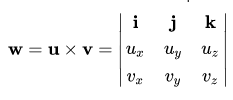
\includegraphics[totalheight=3cm]{img/12.png}
	\end{figure}
	He aquí la implementación:
	\begin{figure}[H]
		\centering
		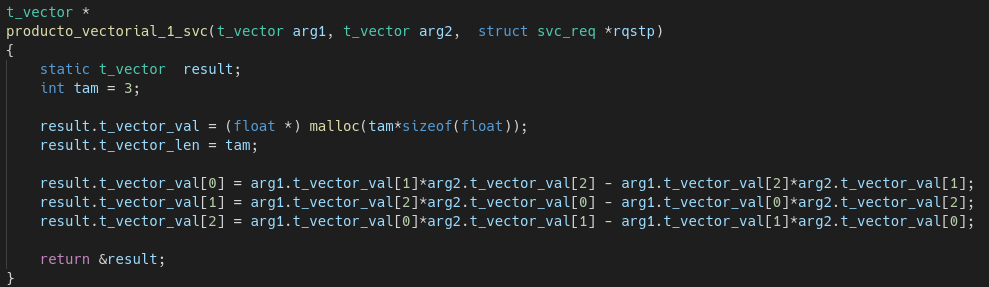
\includegraphics[totalheight=3.5cm]{img/13.png}
	\end{figure}
	El diálogo es parecido a los anteriores, pero no pregunta por la dimensión ya que como hemos mencionado antes, no se puede hacer mayor que 3 (si se quiere hacer de 2 basta con poner 0 en el último componente)
	\begin{figure}[H]
		\centering
		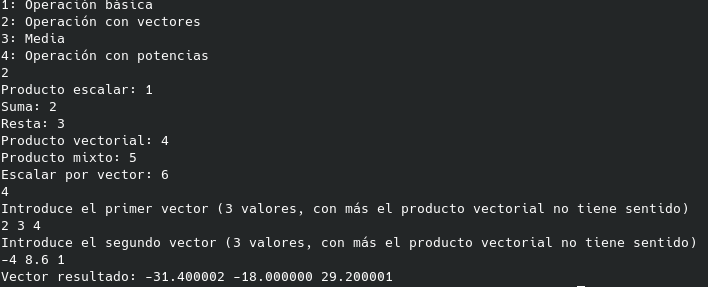
\includegraphics[totalheight=5cm]{img/14.png}
	\end{figure}
	\subsection{Producto mixto}
	Es una combinación del producto escalar y el vectorial, para ello necesitaremos 3 vectores de dimensión 3 máximo. Se calcula el producto vectorial de los dos últimos vectores y luego se hace el producto escalar del primer vector con el vector antes calculado.
	\begin{figure}[H]
		\centering
		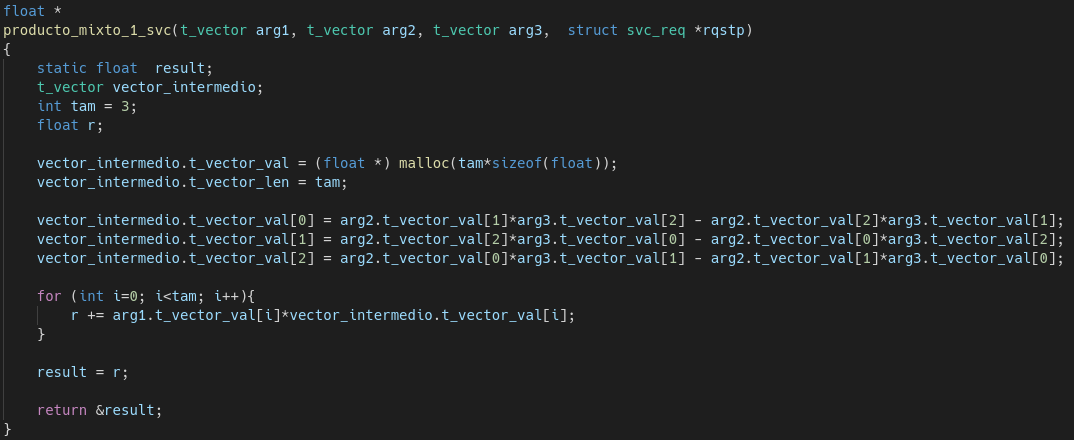
\includegraphics[totalheight=5cm]{img/15.png}
	\end{figure}
	El diálogo es igual al del producto vectorial, pero ahora se piden 3 vectores:
	\begin{figure}[H]
		\centering
		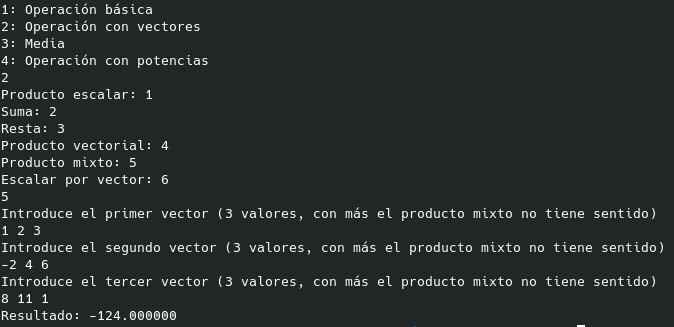
\includegraphics[totalheight=5.8cm]{img/16.png}
	\end{figure}
	\subsection{Producto de un escalar por un vector}
	Simplemente se multiplican todas las coordenadas del vector por dicho escalar.
	\begin{figure}[H]
		\centering
		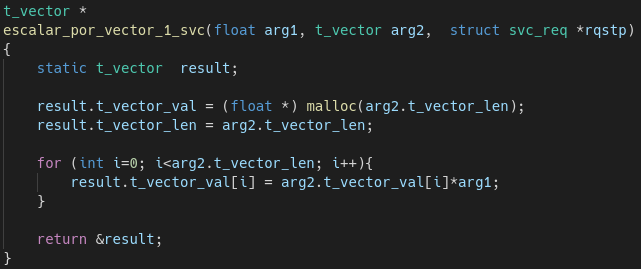
\includegraphics[totalheight=5cm]{img/17.png}
	\end{figure}
	Primero se introducirá la dimensión del vector, luego las componentes de este y por último el escalar.
	\begin{figure}[H]
		\centering
		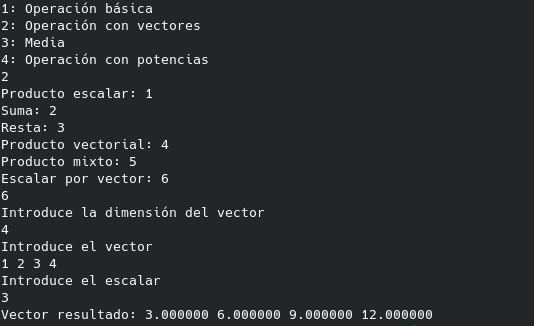
\includegraphics[totalheight=7.5cm]{img/18.png}
	\end{figure}
	\section{Media}
	Esta sección solo contiene una operación, que es realizar la media de un conjunto de reales. Para ello, metemos todos los valores que nos proporciona el usuario en un vector para facilitar el trabajo. He aquí la implementación:
	\begin{figure}[H]
		\centering
		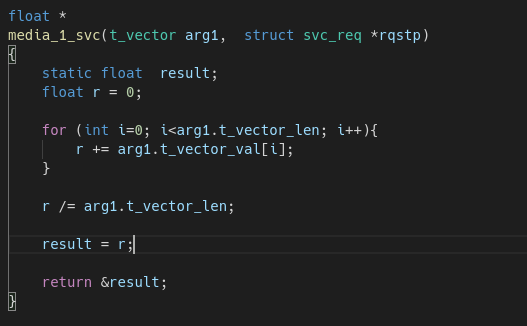
\includegraphics[totalheight=7.7cm]{img/19.png}
	\end{figure}
	Al seleccionar esta opción primero se nos preguntará por el número de valores y luego por los susodichos valores
	\begin{figure}[H]
		\centering
		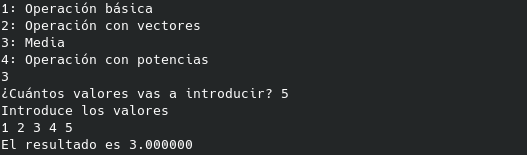
\includegraphics[totalheight=3.7cm]{img/20.png}
	\end{figure}
	\section{Operaciones con potencias}
	Al entrar en esta opción se nos mostrará un pequeño menú con las operaciones a realizar:
	\begin{figure}[H]
		\centering
		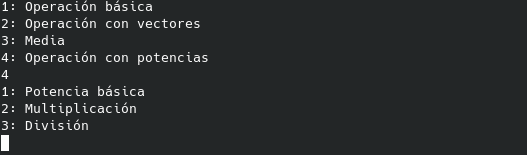
\includegraphics[totalheight=3.7cm]{img/21.png}
	\end{figure}
	Para esta categoría he añadido el struct potencia, que está formado por dos float: base y exponente. Esto facilita el trabajo de base y exponente por separado.
	\subsection{Potencia básica}
	Resuelve una potencia, es decir, eleva la base al exponente, para ello se ha usado pow de math.h.
	\begin{figure}[H]
		\centering
		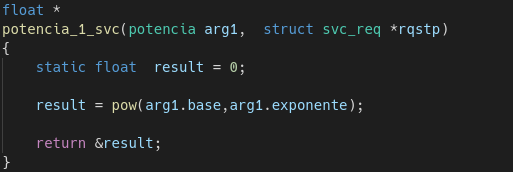
\includegraphics[totalheight=4cm]{img/22.png}
	\end{figure}
	El problema que se ha presentado en esta operación era que el compilador no reconocía pow, para solucionar esto simplemente había que añadir -lm al campo LDLIBS del makefile. He aquí un ejemplo de ejecución:
	\begin{figure}[H]
		\centering
		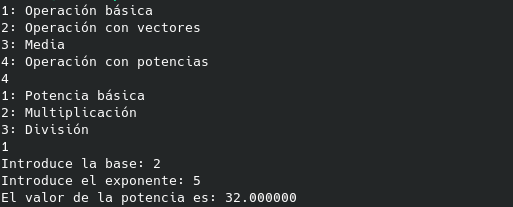
\includegraphics[totalheight=5cm]{img/23.png}
	\end{figure}
	\subsection{Multiplicación de potencias}
	Es necesario para esta función que las potencias tengan la misma base (por ello solo se pide una). Simplemente hay que sumar los exponentes.
	\begin{figure}[H]
		\centering
		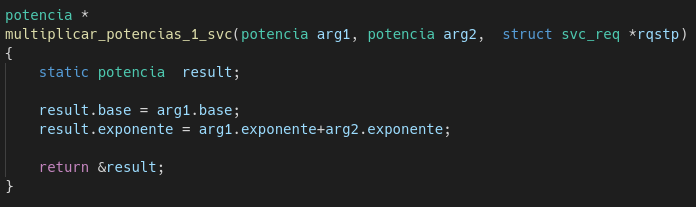
\includegraphics[totalheight=3.7cm]{img/24.png}
	\end{figure}
	Se dará el resultado en forma de base\textasciicircum{}exponente y en forma de número real.
	\begin{figure}[H]
		\centering
		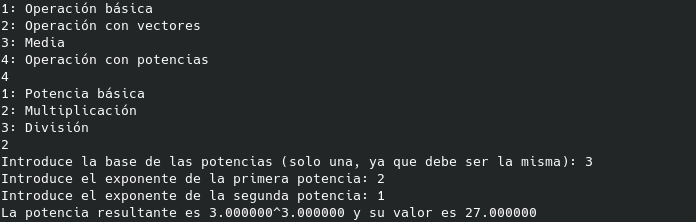
\includegraphics[totalheight=4cm]{img/25.png}
	\end{figure}
	\subsection{División de potencias}
	Igual que la multiplicación pero restamos los exponentes en vez de sumarlos.
	\begin{figure}[H]
		\centering
		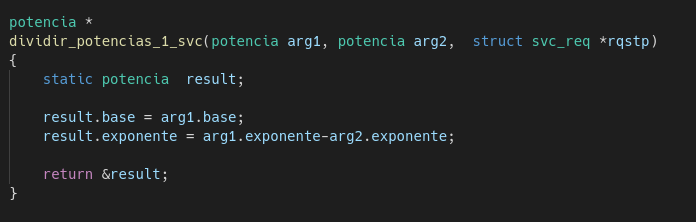
\includegraphics[totalheight=4cm]{img/26.png}
	\end{figure}
	\begin{figure}[H]
		\centering
		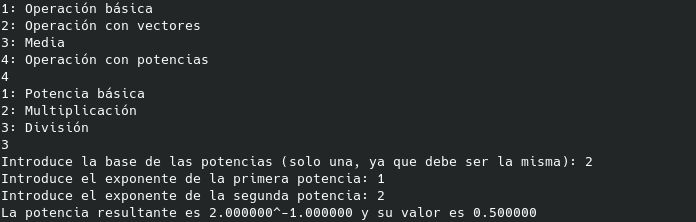
\includegraphics[totalheight=4cm]{img/27.png}
	\end{figure}
\end{document}